\section{Câu 3}
     \hspace*{0.6cm}\textbf{Thực hiện calib camera sau đó so sánh tọa độ thật, độ dài của vật và tọa độ, độ dài của vật tính toán sau khi calib.}
     \subsection{Calib Camera}
          \subsubsection{Mục tiêu}
          \hspace*{0.6cm}Bài tập này nhằm hiệu chỉnh (calibrate) một camera sử dụng mẫu bàn cờ (checkerboard). Thông qua quá trình hiệu chỉnh, ta xác định các tham số nội tại (intrinsic parameters), các hệ số méo ống kính (distortion coefficients) và tham số ngoại tại (extrinsic parameters) mô tả tư thế của bàn cờ trong hệ tọa độ camera. Các tham số này là đầu vào cho các bài toán như hiệu chỉnh méo (undistortion), đo kích thước vật thể, tái tạo 3D, mô phỏng stereo, v.v.

          \subsubsection{Cơ sở lý thuyết}

          \begin{itemize}
               \item \textbf{Mô hình camera lỗ kim}\\
               \hspace*{0.6cm}Mô hình camera đơn giản hóa như một lỗ kim (pinhole), mô tả mối quan hệ giữa không gian 3D và mặt phẳng ảnh 2D.\\
               \hspace*{0.6cm}Công thức chiếu
                    \begin{equation}
                         \begin{bmatrix}
                              s \cdot u \\
                              s \cdot v \\
                              s
                              \end{bmatrix}
                              = K_{int} \ast M_{ext}
                              \begin{bmatrix}
                              X_w \\
                              Y_w \\
                              Z_w \\
                              1
                         \end{bmatrix}
                    \end{equation}
               \hspace*{0.6cm}Trong đó
               \begin{itemize}[label=--]
                    \item $(X_w, Y_w, Z_w)$: Tọa độ điểm trong không gian.
                    \item $(u, v)$: Tọa độ điểm ảnh.
                    \item $K_{int} = 
                    \begin{bmatrix}
                         f_x & 0 & c_x \\
                         0 & f_y & c_y \\
                         0 & 0 & 1
                    \end{bmatrix}$: Ma trận nội tại chứa thông tin tiêu cự, tâm ảnh, hệ số lệch trục.
                    \item $M_{ext} = 
               \begin{bmatrix}
                    R & t \\
                    0_{1 \times 3} & 1
               \end{bmatrix}$: Ma trận thông số ngoại dùng để chuyển tọa độ vật từ tọa độ toàn cục về tọa độ camera.
               \end{itemize}
               \item \textbf{Méo hình của ống kính}
               \begin{itemize}
                    \item Ống kính thực gây ra méo hình so với mô hình lý tưởng. Có hai loại méo chính:
                    \begin{itemize}[label=+]
                         \item \textbf{Méo hướng tâm (radial):} làm các đường thẳng gần rìa bị cong, được mô tả bởi các hệ số $k_1, k_2, k_3$.
                         \item \textbf{Méo tiếp tuyến (tangential):} do ống kính lắp lệch tâm hoặc cảm biến bị nghiêng, mô tả bởi $p_1, p_2$.
                    \end{itemize}
                    \item OpenCV gom các hệ số này trong vector:
                                   \begin{equation}
                    dist = [k_1, k_2, p_1, p_2, k_3, \ldots]
               \end{equation}
               \end{itemize}

               \item \textbf{Bài toán hiệu chỉnh camera}\\
               \hspace*{0.6cm}Cho nhiều ảnh bàn cờ, mỗi ảnh ta có:
               \begin{itemize}[label=--]
                    \item \textbf{Object points:} tọa độ 3D các góc nội của bàn cờ, biết trước trong đơn vị mm.
                    \item \textbf{Image points:} tọa độ 2D (u, v) của các góc nội tương ứng trên ảnh.
               \end{itemize}
               \hspace*{0.6cm}Hàm \texttt{cv2.calibrateCamera} sẽ tìm $K$, $dist$, cùng với $R_i, t_i$ cho từng ảnh sao cho lỗi chiếu lại (reprojection error) giữa các điểm ảnh quan sát và các điểm ảnh dự đoán là nhỏ nhất. Giá trị RMS càng nhỏ thì kết quả hiệu chỉnh càng chính xác.
          \end{itemize}
          

          \subsubsection{Các bước thực hiện}

          \hspace*{0.6cm}\textbf{Camera:} camera số chụp ảnh tĩnh. Mẫu bàn cờ được in trên giấy, dán lên mặt phẳng cứng như Hình~\ref{s3_p01_origin_checkerboard}. Sử dụng số góc nội \texttt{CHECKERBOARD} = (7, 10). Cạnh mỗi ô vuông có kích thước \texttt{square\_size\_mm} = 25 mm.\\
          \hspace*{0.6cm}Bộ ảnh hiệu chỉnh gồm nhiều ảnh bàn cờ được chụp ở các tư thế và khoảng cách khác nhau, giúp dữ liệu phong phú và phủ đều cảm biến. Ở đây nhóm sử dụng 25 ảnh bàn cờ để thực hiện hiệu chỉnh.

          \begin{figure}[H]
               \centering
               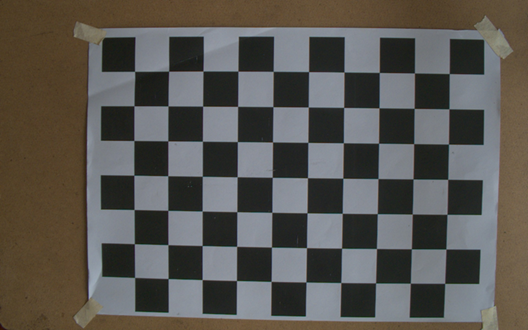
\includegraphics[width=0.6\textwidth]{pictures/section3/s3_p01_origin_checkerboard.png}
               \caption{Ảnh bàn cờ gốc dùng cho hiệu chỉnh camera.}
               \label{s3_p01_origin_checkerboard}
          \end{figure}

          \begin{itemize}
               \item \textbf{Bước 1:} Xây dựng hệ tọa độ bàn cờ (object points).\\
               \hspace*{0.6cm}Ta giả sử toàn bộ bàn cờ nằm trên mặt phẳng $Z = 0$. Gốc tọa độ $(0, 0, 0)$ đặt tại một góc nội của bàn cờ. Trục $X$ chạy theo chiều ngang bàn cờ, trục $Y$ theo chiều dọc. Sử dụng \texttt{np.mgrid} sinh ra lưới các chỉ số $(0 \ldots 6, 0 \ldots 9)$, sau đó nhân với kích thước ô vuông 25 mm để thu được 70 điểm 3D.\\
               \hspace*{0.6cm}Lưới object points này là như nhau cho mọi ảnh, vì hình học bàn cờ không đổi. Mỗi ảnh sẽ dùng cùng một tập object points và một tập image points riêng.
               \item \textbf{Bước 2:} Tìm các góc bàn cờ trên ảnh (image points).\\
               \hspace*{0.6cm}Các ảnh trong thư mục được lần lượt đọc và chuyển sang ảnh xám. Hàm \texttt{cv2.findChessboardCorners} với kích thước (7, 10) được sử dụng để tìm vị trí các góc nội. Nếu nhận diện thành công (\texttt{ret = True}), vị trí góc được refine bằng \texttt{cv2.cornerSubPix} để đạt độ chính xác sub-pixel.\\
               \hspace*{0.6cm}Kết quả refine được đưa vào \texttt{imgpoints}, trong khi object points tương ứng được đưa vào \texttt{objpoints}. Đồng thời, chương trình vẽ các góc lên ảnh bằng \texttt{cv2.drawChessboardCorners} và lưu lại, giúp kiểm tra trực quan xem việc phát hiện góc có chính xác hay không.
               \begin{figure}[H]
                    \centering
                    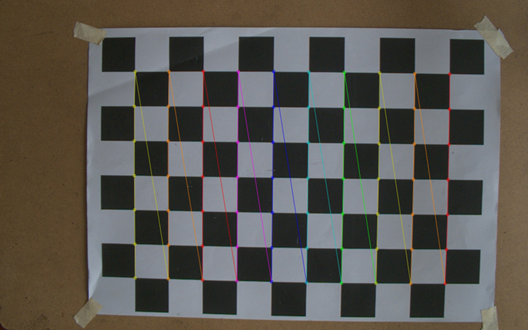
\includegraphics[width=0.6\textwidth]{pictures/section3/s3_p02_checkerboard_afterOpCV.png}
                    \caption{Ảnh bàn cờ sau khi phát hiện và nối các góc nội bằng OpenCV.}
                    \label{s3_p02_checkerboard_afterOpCV}
               \end{figure}
               \item \textbf{Bước 3:} Gọi \texttt{cv2.calibrateCamera} và \texttt{cv2.getOptimalNewCameraMatrix} để tính các tham số nội tại, ngoại tại và hệ số méo.\\
               \hspace*{0.6cm}Sau khi thu đủ dữ liệu, ta gọi \texttt{cv2.calibrateCamera(objpoints, imgpoints, (w, h), ...)} để tính các tham số nội tại và ngoại tại. Kết quả chính trong thí nghiệm là:
               \begin{itemize}[label=--]
                    \item Reprojection error (RMS) $\approx$ 0.499977 pixel (xấp xỉ 0.50 pixel).
                    \item Ma trận nội tại $K$:
               \end{itemize}
               \begin{equation}
                    K = \begin{bmatrix}
                         2385.3882 & 0.0000 & 944.8986 \\
                         0.0000 & 2387.7920 & 553.7859 \\
                         0.0000 & 0.0000 & 1.0000
                    \end{bmatrix}
               \end{equation}
               \hspace*{0.6cm}Suy ra:
               \begin{align*}
                    f_x &= 2385.3882 \text{ pixel} \\
                    f_y &= 2387.7920 \text{ pixel} \\
                    c_x &= 944.8986 \text{ pixel} \\
                    c_y &= 553.7859 \text{ pixel}
               \end{align*}
               \hspace*{0.6cm}$f_x$ và $f_y$ gần bằng nhau, cho thấy pixel gần vuông. Tâm ảnh $(c_x, c_y)$ nằm gần trung tâm khung hình, phù hợp với cấu trúc cảm biến của camera.\\
               \hspace*{0.6cm}Vector hệ số méo thu được là:
               \begin{equation}
                    dist = [k_1, k_2, p_1, p_2, k_3] = [-0.202966, -0.000392, 0.000621, 0.001218, 0.975811]
               \end{equation}
               \hspace*{0.6cm}Trong đó $k_1, k_2$ âm thể hiện méo dạng barrel nhẹ; $k_3$ dương mô tả méo bậc cao hơn; $p_1, p_2$ rất nhỏ nên méo tiếp tuyến không đáng kể.
               \begin{figure}[H]
                    \centering
                    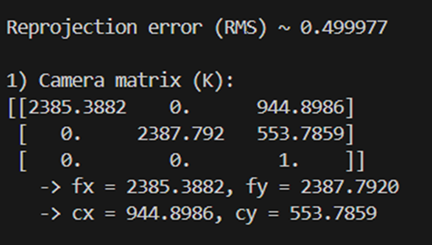
\includegraphics[width=0.7\textwidth]{pictures/section3/s3_p03_RMS_insK.png}
                    \caption{Kết quả in ra màn hình: sai số RMS và ma trận nội tại K.}
                    \label{s3_p03_RMS_insK}
               \end{figure}
               \begin{figure}[H]
                    \centering
                    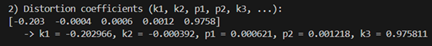
\includegraphics[width=0.7\textwidth]{pictures/section3/s3_p04_distortion.png}
                    \caption{Kết quả các hệ số méo (distortion coefficients).}
                    \label{s3_p04_distortion}
               \end{figure}
               \begin{figure}[H]
                    \centering
                    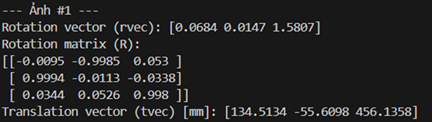
\includegraphics[width=0.7\textwidth]{pictures/section3/s3_p05_ext.png}
                    \caption{Tham số ngoại tại cho ảnh bàn cờ 1.}
                    \label{s3_p05_ext}
               \end{figure}
               \item \textbf{Nhận xét:}\\
               \hspace*{0.6cm}Giá trị $RMS \approx 0.42$ pixel cho thấy kết quả hiệu chỉnh là tốt; sai số chiếu lại trung bình nhỏ hơn một pixel. Ma trận nội tại thu được hợp lý, tâm ảnh gần trung tâm khung hình. Các hệ số méo có trị số vừa phải, chứng tỏ ống kính có méo nhưng không quá nghiêm trọng và hoàn toàn có thể hiệu chỉnh bằng các hàm undistort của OpenCV.
               \hspace*{0.6cm}Một số nguồn sai số có thể tồn tại:
               \begin{itemize}[label=--]
                    \item Bàn cờ in trên giấy có thể bị cong hoặc nhăn.
                    \item Một số ảnh có ánh sáng không đồng đều, làm giảm tương phản ô đen -- trắng.
                    \item Số lượng và độ đa dạng của ảnh có thể chưa tối ưu; nếu nhiều ảnh có góc chụp gần giống nhau thì thông tin hình học thu được không phong phú.
               \end{itemize}
               \hspace*{0.6cm}Để cải thiện, có thể tăng số ảnh, thay đổi nhiều hơn về góc nhìn và khoảng cách, sử dụng vật liệu in cứng và loại bỏ các ảnh bị mờ hoặc thiếu sáng.
          \end{itemize}
     \subsection{Tính Độ Dài Vật}
          \subsubsection{Mục tiêu bài tập}
          \hspace*{0.6cm}Trong bài thực hành này, mục tiêu là sử dụng kết quả hiệu chỉnh (calibration) của camera để đo kích thước thực của một vật thể phẳng đặt trên cùng mặt phẳng với bàn cờ hiệu chỉnh. Cụ thể, chương trình cần:
          \begin{itemize}
               \item Chuyển bốn góc từ toạ độ pixel sang toạ độ thế giới (mm) dựa trên các tham số nội/ngoại của camera.
               \item Tính chiều dài, chiều rộng thực tế của thẻ và so sánh với số đo bằng thước thực tế.
          \end{itemize}
          \subsubsection{Cơ sở lý thuyết}
               \begin{itemize}
                    \item \textbf{Mô hình chiếu phối cảnh camera}\\
                    \hspace*{0.6cm}Quan hệ giữa điểm trong không gian thế giới $M_w = [X_w, Y_w, Z_w]^T$ và điểm trong hệ toạ độ camera $M_c = [X_c, Y_c, Z_c]^T$ được mô tả bởi:
                         \begin{equation}
                         M_c = R \cdot M_w + T
                         \end{equation}
                    \hspace*{0.6cm}Trong đó $R$ $(3 \times 3)$ là ma trận quay và $T$ $(3 \times 1)$ là vector tịnh tiến từ hệ thế giới sang hệ camera (được lấy từ file hiệu chỉnh).\\
                    \hspace*{0.6cm}Từ hệ camera sang điểm ảnh (pixel), ta có quan hệ chiếu phối cảnh: $s \cdot m_p = K \cdot M_c$, với $m_p = [u, v, 1]^T$ là toạ độ pixel ở dạng đồng nhất, $K$ là ma trận nội chứa các tham số tiêu cự và tâm ảnh.
                    \item \textbf{Chuyển tọa độ pixel sang tọa độ thế giới trên mặt phẳng $Z_w = 0$}\\
                    \hspace*{0.6cm}Nếu giả sử vật thể nằm trên mặt phẳng $Z_w = 0$ (mặt phẳng bàn cờ), ta có thể tính ngược toạ độ thế giới từ pixel. Từ $s \cdot m_p = K \cdot (R \cdot M_w + T)$, kết hợp với điều kiện $Z_w = 0$, ta suy ra:
                         \begin{equation}
                         M_w = R^{-1} (K^{-1} \cdot z_{cam} \cdot m_p - T)
                         \end{equation}
                    \hspace*{0.6cm}Trong chương trình, $z_{cam}$ (độ sâu trong hệ camera) được tính bằng cách xét thành phần thứ ba (trục $Z_w$) của $M_w$ và ép điều kiện $Z_w = 0$ để giải ra $z_{cam}$. Sau đó, $M_w$ được tính lại bằng công thức trên, cho ta toạ độ $(X_w, Y_w, Z_w)$ tính theo mm.
               \end{itemize}             
          \subsubsection{Các bước thực hiện}
               \begin{itemize}
                    \item \textbf{Camera:} camera đã được hiệu chỉnh trước đó bằng phương pháp Zhang với bàn cờ chuẩn $7 \times 10$ góc nội.
                    \item \textbf{File tham số hiệu chỉnh:} \texttt{calib\_params.json}, lưu ma trận nội $K$ và các cặp (\texttt{rvec}, \texttt{tvec}) cho nhiều tư thế chụp bàn cờ.
                    \item \textbf{Vật đo:} thẻ quảng cáo giấy, kích thước thực tế xấp xỉ 90 mm $\times$ 54 mm (quan sát bằng thước).
               \end{itemize}

               \begin{figure}[H]
                    \centering
                    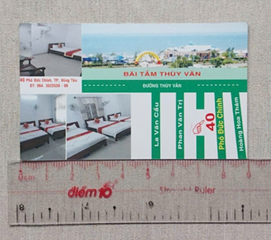
\includegraphics[width=0.6\textwidth]{pictures/section3/s3_p06_obj_length.png}
                    \caption{Thẻ quảng cáo và thước đo -- bố trí theo chiều dài.}
                    \label{s3_p06_obj_length}
               \end{figure}

               \begin{figure}[H]
                    \centering
                    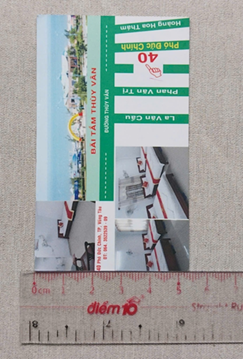
\includegraphics[width=0.5\textwidth]{pictures/section3/s3_p07_obj_width.png}
                    \caption{Thẻ và thước đo -- bố trí theo chiều rộng.}
                    \label{s3_p07_obj_width}
               \end{figure}
               \begin{itemize}
                    \item \textbf{Bước 1. Đọc tham số hiệu chỉnh từ file JSON}\\
                    \hspace*{0.6cm}Sau khi calib các thông số được lưu vào file JSON. Hàm \texttt{load\_calib()} đọc ma trận nội $K$, danh sách \texttt{rvecs} và \texttt{tvecs} từ \texttt{calib\_params.json}. Vector quay \texttt{rvec} được chuyển sang ma trận quay $R$ bằng hàm \texttt{cv2.Rodrigues()}. Từ đó, ta thu được bộ tham số $(K, R, T)$ ứng với một tư thế camera (\texttt{POSE\_INDEX}).
                    \item \textbf{Bước 2. Tiền xử lý ảnh và nhị phân hoá}\\
                    \hspace*{0.6cm}Ảnh màu được chuyển sang mức xám, làm mượt bằng \texttt{GaussianBlur} để giảm nhiễu. Sau đó, dùng phân ngưỡng Otsu (\texttt{cv2.THRESH\_OTSU}) để tách nền -- vật thể, thu được ảnh nhị phân. Các phép hình thái học mở (opening) và đóng (closing) với kernel $3 \times 3$ được áp dụng để loại nhiễu nhỏ và làm đầy các lỗ hổng trong vùng thẻ.
                    \item \textbf{Bước 3. Tìm contour lớn nhất và hình chữ nhật bao nhỏ nhất}\\
                    \hspace*{0.6cm}Dùng \texttt{cv2.findContours()} với chế độ \texttt{RETR\_EXTERNAL} để lấy các contour ngoài cùng. Contour có diện tích lớn nhất được giả định là thẻ cần đo. Hàm \texttt{cv2.minAreaRect()} được dùng để tìm hình chữ nhật bao nhỏ nhất (min-area rectangle) cho contour này, trả về toạ độ tâm, kích thước $(w, h)$ và góc xoay. Từ đó, \texttt{cv2.boxPoints()} cho ta bốn đỉnh của hình chữ nhật này trong hệ pixel.
                    \item \textbf{Bước 4. Chuyển bốn góc từ pixel sang toạ độ thế giới}\\
                    \hspace*{0.6cm}Bốn điểm góc $(u, v)$ thu được từ \texttt{boxPoints()} được truyền vào hàm \\
                    \texttt{pixel\_to\_world\_on\_plane()}. Hàm này triển khai công thức nghịch $M_w = R^{-1}(K^{-1} \cdot z_{cam} \cdot m_p - T)$, trong đó $z_{cam}$ được giải bằng cách áp điều kiện $Z_w = 0$. Kết quả là toạ độ $(X_w, Y_w, Z_w)$ của từng góc trong hệ thế giới, đơn vị mm.
                    \item \textbf{Bước 5. Tính chiều dài và chiều rộng thẻ}\\
                    \hspace*{0.6cm}Sau khi có bốn điểm trong không gian thế giới, khoảng cách giữa các cặp đỉnh liên tiếp được tính bằng chuẩn Euclid. Trong bốn cạnh, cạnh dài nhất được coi là chiều dài, cạnh ngắn nhất là chiều rộng của thẻ. Các giá trị này là kết quả đo kích thước thực tế dựa trên hiệu chỉnh camera.
               \end{itemize}
          \subsubsection{Kết quả thực nghiệm}
               \begin{itemize}
                    \item \textbf{Toạ độ bốn góc trong hệ pixel}\\
                    \hspace*{0.6cm}Bốn góc của thẻ trong ảnh (theo thứ tự \texttt{boxPoints}) được hiển thị trong Hình~\ref{s3_p09_obj_coor_4_cor}.
                    \begin{figure}[H]
                         \centering
                         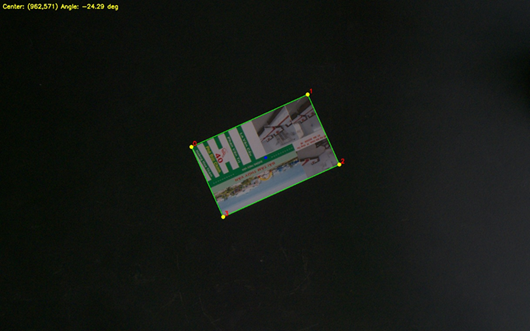
\includegraphics[width=0.5\textwidth]{pictures/section3/s3_p08_obj_detect_4_cor.png}
                         \caption{Hình ảnh phát hiện 4 góc của hình.}
                         \label{s3_p08_obj_detect_4_cor}
                    \end{figure}
                    \begin{figure}[H]
                         \centering
                         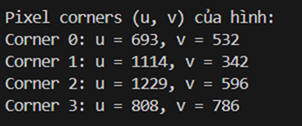
\includegraphics[width=0.7\textwidth]{pictures/section3/s3_p09_obj_coor_4_cor.png}
                         \caption{Hình ảnh tọa độ pixel 4 góc.}
                         \label{s3_p09_obj_coor_4_cor}
                    \end{figure}
                    \item \textbf{Toạ độ bốn góc trong hệ thế giới (mm)}\\
                    \hspace*{0.6cm}Sau khi chuyển đổi sang hệ toạ độ thế giới trên mặt phẳng $Z_w = 0$, ta thu được kết quả trong Hình~\ref{s3_p10_obj_coor_4_cors_world}.
                    \begin{figure}[H]
                         \centering
                         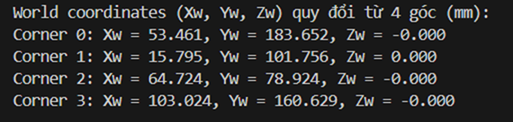
\includegraphics[width=0.7\textwidth]{pictures/section3/s3_p10_obj_coor_4_cors_world.png}
                         \caption{Hình ảnh quy đổi tọa độ thực 4 góc.}
                         \label{s3_p10_obj_coor_4_cors_world}
                    \end{figure}
                    \item \textbf{Kích thước ước lượng của thẻ tính theo Euclid}\\
                    \hspace*{0.6cm}Khoảng cách giữa các cặp góc liên tiếp được tính bằng công thức Euclid:
                    \begin{figure}[H]
                         \centering
                         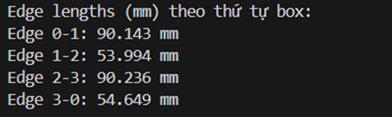
\includegraphics[width=0.7\textwidth]{pictures/section3/s3_p11_obj_edge_length.png}
                         \caption{Độ dài các cạnh.}
                         \label{s3_p11_obj_edge_length}
                    \end{figure}
                    \begin{figure}[H]
                         \centering
                         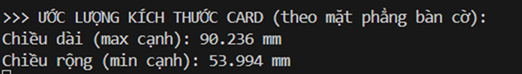
\includegraphics[width=0.7\textwidth]{pictures/section3/s3_p12_obj_final_length.png}
                         \caption{Kích thước cuối cùng của vật.}
                         \label{s3_p12_obj_final_length}
                    \end{figure}
                    \item \textbf{So sánh với số đo thực tế}\\
                    \hspace*{0.6cm}Dựa trên hình ảnh thước đo kèm theo (Hình~\ref{s3_p06_obj_length} và Hình~\ref{s3_p07_obj_width}), kích thước thực của thẻ xấp xỉ: chiều dài 90 mm và chiều rộng 54 mm. So sánh với kết quả đo bằng camera:
                    \begin{itemize}
                         \item \textbf{Chiều dài:} 90.236 mm so với 90 mm $\rightarrow$ sai số khoảng 0.236 mm ($\sim$0.26\%).
                         \item \textbf{Chiều rộng:} 53.994 mm so với 54 mm $\rightarrow$ sai số khoảng 0.006 mm ($\sim$0.01\%).
                    \end{itemize}
                    Sai số rất nhỏ, cho thấy quá trình hiệu chỉnh và đo đạc hoạt động tốt.  
               \end{itemize}
  
               

